\apendice{Documentación técnica de programación}

\section{Introducción}
Esta sección describe la documentación técnica de programación, incluyendo la instalación del entorno de desarrollo, la estructura de directorios, la estrutura de la aplicación y su compilación.
\section{Estructura de directorios}
El repositorio del proyecto se distribuye de la siguiente manera:

\begin{itemize}
    \item \textbf{/}:
    \begin{itemize}
        \item \texttt{.gitignore}: Archivo que especifica qué archivos y directorios deben ser ignorados por Git.
        \item \texttt{LICENSE}: Copia de la licencia MIT.
        \item \texttt{README.md}: archivo que describe la estructura y detalles del proyecto.
    \end{itemize}
    \item \textbf{/Codigos/Angular/proyecto/}:
    \begin{itemize}
        \item \textbf{Proyecto Angular}: Contiene el código del proyecto Angular junto con los ficheros de configuración del proyecto y el archivo de dependencias.
        \item \textbf{/dist/}: Archivos para la puesta en producción de la aplicación Angular.
        \item \textbf{/src/}:
        \begin{itemize}
            \item \textbf{Código fuente}: Contiene el código fuente de la aplicación Angular junto con su estructura general de ficheros.
            \item \textbf{/assets/img/}: Imágenes y vídeos utilizados en la aplicación web.
            \item \textbf{/app/}:
            \begin{itemize}
                \item \textbf{Módulos compartidos}: Componentes compartidos como el \texttt{header} y el \texttt{footer}.
                \item \textbf{Servicios}: Servicios de la aplicación que se encargan de realizar las llamadas a las APIs.
                \item \textbf{Componente login}: Inicio de sesión con Google.
                \item \textbf{Interfaces}: Conjunto de interfaces utilizadas en el desarrollo.
                \item \textbf{Guards}: Protección de rutas en Angular.
                \item \textbf{Módulo \texttt{aplicacion}}: Contiene el resto de componentes de la aplicación.
                \item \textbf{/aplicacion/pages}: Componentes que forman las vistas de la aplicación:
                \begin{itemize}
                    \item \textbf{Competiciones}: Vista de competiciones.
                    \item \textbf{Equipos}: Vista de equipos.
                    \item \textbf{Goles Esperados}: Vista de goles esperados.
                    \item \textbf{Inicio}: Vista de inicio.
                    \item \textbf{Mundial}: Vista del mundial.
                    \item \textbf{Partidos}: Vista de partidos.
                    \item \textbf{Predicciones}: Vista de predicciones.
                    \item \textbf{Sport-IA}: Vista de sport-IA.
                    \item Cada directorio contiene sus respectivos ficheros HTML, CSS y TypeScript.
                \end{itemize}
            \end{itemize}
        \end{itemize}
    \end{itemize}
    \item \textbf{/Codigos/Flask/}:
    \begin{itemize}
        \item \textbf{Aplicación Flask}: Contiene la aplicación de Flask.
        \item \textbf{/static/}: Guarda las imágenes generadas.
        \item \textbf{/uploads/}: Guarda los vídeos procesados por imageAI.
        \item \textbf{Distintos ficheros JSON}: Contienen los resultados de los modelos de predicción.
        \item \textbf{/flaskApp/}:
        \begin{itemize}
            \item \textbf{Ficheros Python}: Desarrollados para generar el modelo de goles esperados, modelo de puntos esperados, gráficas del mundial y procesado de vídeo con imageAI.
            \item \texttt{routes.py}: Contiene las rutas definidas en la aplicación Flask.
        \end{itemize}
    \end{itemize}
    \item \textbf{/Memoria/}:
    \begin{itemize}
        \item \textbf{Documentación del proyecto}: Contiene la memoria y los anexos del proyecto en LaTeX y en formato \texttt{.pdf}.
        \item \textbf{/img/}: Imágenes utilizadas en la documentación.
    \end{itemize}
    \item \textbf{/Prototipos/}:
    \begin{itemize}
        \item \texttt{Prototipos 1.0.vp}: Fichero que contiene los prototipos realizados con la aplicación \texttt{JustInMind}.
    \end{itemize}
\end{itemize}

\section{Manual del programador}
El siguiente manual tiene como objetivo servir de referencia para futuros desarrolladores que trabajen en la aplicación. En él, se detalla como montar el entorno de desarrollo, obtener el código fuente del proyecto, instalarlo, compilarlo y ejecutarlo en local.
\subsection{Entorno de desarrollo}
Para trabajar con el proyecto se necesita tener instalados los siguientes programas:
\begin{itemize}
    \item Visual Studio Code.
    \item Node.js
    \item Git
    \item Python 3.8
    \item Angular
\end{itemize}

\subsubsection{Visual Studio Code}
Visual Studio Code es un editor de código fuente gratuito, multiplataforma desarrollado por Microsoft. Se ha convertido en una de las herramientas de desarrollo más populares debido a su versatilidad (permite una amplia variedad de lenguajes de programación), rendimiento y amplio conjunto de características. Su integración con Git facilita el control de versiones, revisión del código y la colaboración en equipo. Podemos descargar Visual Studio Code desde su página oficial \cite{visualStudioCode:latex} eligiendo el sistema operativo y la arquitectura del ordenador y, posteriormente, seguir el asistente de instalación.

\subsubsection{Node.js}
Node.js es un entorno de ejecución JavaScript que permite a los desarrolladores ejecutar código JavaScript del lado del servidor. Node.js incluye npm, que es la herramienta de gestión de paquetes más utilizada en el ecosistema de JavaScript. Angular y sus dependencias se distribuyen a través de npm, por lo que es esencial tener Node.js instalado para poder instalar Angular y sus bibliotecas asociadas. Se puede descargar la versón de Node.js desde su página oficial y seguir los pasos del instalador \cite{nodejs:latex}.

\subsubsection{Git}
Para poder hacer uso del repositorio en GitHub es necesario tener instalado el gestor de versiones Git. Este programa nos permitirá clonar el repositorio, movernos por sus ramas. Se puede obtener desde \cite{git:latex}.

\subsubsection{Python}
Python es un lenguaje de programación muy popular para realizar cualquier tipo de programa, o aplicación utilizando microframeworks como Flask. Antes de instalar Flask, es necesario tener instalada la versión de Python 3.8.0 debido a que algunas de las dependencias utilizadas requieren de esta versión de Python para funcionar correctamente. \\
Para instalar Python 3.8.0 se puede hacer desde \cite{python:latex} y seguir los pasos del instalador.

\subsubsection{Angular}
Angular es un framework de aplicaciones web de código abierto desarrollado por Google. Está diseñado para facilitar la creación de aplicaciones web dinámicas de una sola página. Angular permite a los desarrolladores construir aplicaciones web modernas con una arquitectura robusta y un código mantenible. \\
Para instalar Angular, es necesario tener Node.js y npm instalados en tu sistema, debido a que el Angular CLI (\textit{Command Line Interface}) se distribuye a través de npm. \\
Una vez instalado Node.js y npm (se instala al instalar Node.js), podremos pasar a instalar Angular en nuestro sistema utilizando el comando '\textit{npm install -g @angular/cli}' en una ventana de comandos. \\
Una vez instalado, podremos comprobar que se ha instalado con éxito ejecutando el comando 'ng version' como se puede ver en la figura. \\
Podemos obtener más información en la página oficial de Angular \cite{Angular:latex}.
\begin{figure}[H]
    \centering
    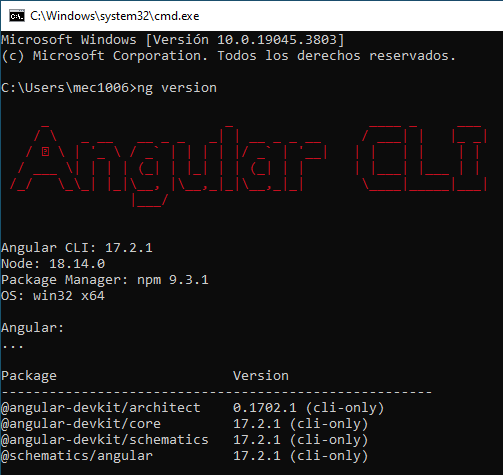
\includegraphics[width=0.65\linewidth]{img/angularInstalacion.png}
    \caption{Ejecución de \textit{ng version} para comprobar la instalación.}
    \label{fig:enter-label}
\end{figure}
\section{Compilación, instalación y ejecución del proyecto}
\subsection{Obtención del código fuente del repositorio}
Para el desarrollo de la aplicación se ha utilizado un repositorio Git hospedado en GitHub. Para obtener una copia de este hay que proceder de la siguiente manera:
\begin{enumerate}
    \item Abrir la terminal Git Bash.
    \item Desplazarse utilizando el comando cd al directorio donde deseemos copiar el repositorio.
    \item Introducir el siguiente comando: \\
    \textbf{git clone https://github.com/MiguelExtremo/TFG.git}
    \item Se iniciará la descarga del repositorio, cuando finalice se dispondrá de una copia de este.
\end{enumerate}

\begin{figure}[H]
    \centering
    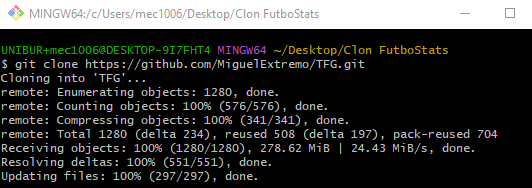
\includegraphics[width=0.75\linewidth]{img/clonarRepo.png}
    \caption{Clonar repositorio de GitHub.}
    \label{fig:enter-label}
\end{figure}
Para más información sobre el proceso de clonar repositorios se puede consultar \cite{clonar:latex}.

\subsection{Importar proyecto en Visual Studio Code}
Una vez clonado el repositorio y con el código fuente de la aplicación, lo importamos en Visual Studio Code siguiendo los siguientes pasos:
\begin{enumerate}
    \item Abrir Visual Studio Code
    \item Menú File > Open folder
    \item Buscamos el directorio donde hemos clonado el repositorio.
    \item Abrimos el directorio en Visual Studio Code.
\end{enumerate}
Una vez importado el proyecto en Visual Studio Code pasaremos a explicar como instalar las dependencias de Angular y las dependencias de Flask.
\begin{figure}[H]
    \centering
    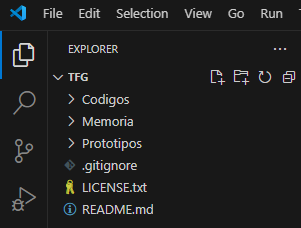
\includegraphics[width=0.55\linewidth]{img/importarVSC.png}
    \caption{Importar proyecto en Visual Studio Code}
    \label{fig:enter-label}
\end{figure}

\subsection{Instalar dependencias de Angular}
Para instalar las dependencias de Angular necesitamos generar la carpeta 'node modules'. Este directorio es el más importante en proyectos Angular, ya que contiene todos los módulos y paquetes que el proyecto necesita para funcionar. Cada vez que se instalan dependencias nuevas en un proyecto Angular usando npm, se descargan y se almacenan en la carpeta 'node modules'. \\
Todos los paquetes y módulos de terceros especificados en el archivo 'package.json' del proyecto se descargan y almacenan en la carpeta 'node modules'. Esto incluye bibliotecas de Angular, utilidades de desarrollo, herramientas de construcción, y cualquier otra dependencia que la aplicación requiera.

Para crear la carpeta node modules se deben seguir los siguientes pasos:
\begin{enumerate}
    \item Abrir la terminal en la raíz del proyecto Angular.
    \item Ejecutar el comando \\
    \textbf{npm install}
    \item Se descargarán todas las dependencias listadas en 'package.json' y creará la carpeta 'node modules'.
\end{enumerate}

Este comando puede tardar varios minutos en terminar de ejecutarse. Una vez termine podremos ver la carpeta node modules creada en la raíz del proyecto.
\begin{figure}[H]
    \centering
    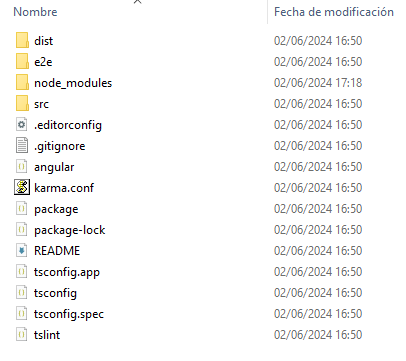
\includegraphics[width=0.6\linewidth]{img/nodemodules.png}
    \caption{Creación de la carpeta node modules con las dependencias del proyecto Angular}
    \label{fig:enter-label}
\end{figure}

\subsection{Creación entorno virtual para la aplicación Flask}
Crear un entorno virtual es una buena práctica para mantener las dependencias del proyecto aisladas de otras en el sistema. Para crear un entorno virtual y activarle se siguen los siguientes pasos:
\begin{enumerate}
    \item Abrir una ventana de comandos en el directorio donde queramos crear el entorno virtual.
    \item Ejecutar el comando: \\
    \textbf{python -m venv venv}
    \item El comando creará un entorno virtual en un directorio llamado 'venv'.
    \item Una vez creado nos movemos con cd a venv/Scripts/activate.
    \item Veremos que el prompt cambia para indicar que el entorno virtual está activado.
\end{enumerate}
\begin{figure}[H]
    \centering
    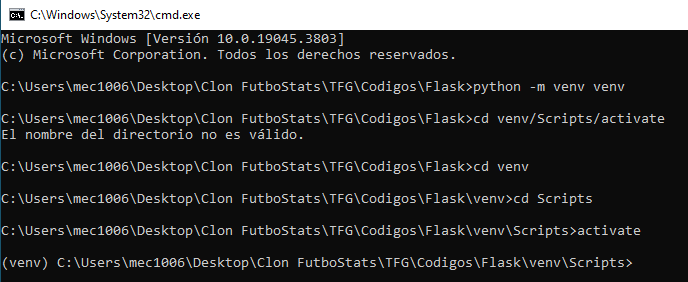
\includegraphics[width=0.75\linewidth]{img/entornoVirtual.png}
    \caption{Creación y activación del entorno virtual en Python.}
    \label{fig:enter-label}
\end{figure}

\subsection{Instalar las dependecias del proyecto Flask}
Con el entorno virtual activado seguimos los siguientes pasos:
\begin{enumerate}
    \item Navegamos con cd al directorio donde se encuentra el fichero 'requirements.txt'.
    \item Ejecutamos el siguiente comando para instalar las dependencias:\\
    \textbf{pip install -r requirements.txt}
    \item Como resultado habremos instalado las dependencias del proyecto de Flask.
    \item Ejecutar comando 'pip list' para comprobar que se han instalado las dependencias.
\end{enumerate}
Este proceso de instalación de las dependencias del proyecto Flask puede tardar unos minutos. \\
\begin{figure}[H]
    \centering
    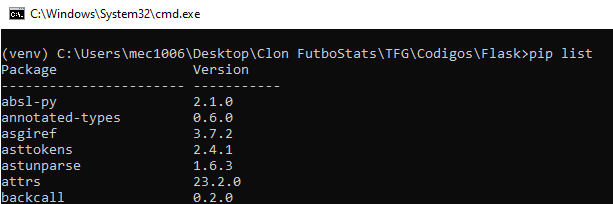
\includegraphics[width=0.75\linewidth]{img/listarDependencias.png}
    \caption{Listar dependencias instaladas utilizando el comando \textit{pip list}.}
    \label{fig:enter-label}
\end{figure}
\subsection{Otras instalaciones: Ffmpeg}
Para poder utilizar la herramienta ImageAI sin problemas e integrarla en una aplicación web es necesario instalar la herramienta Ffmpeg. Es un programa utilizado para codificar los formatos de los vídeos que el usuario introduce. Si no se instala este programa, el vídeo procesado por ImageAI y devuelto a la aplicación web no podrá visualizarse correctamente debido a que la codificación de el vídeo no es compatible con los navegadores.
Para instalar la herramienta solo hay que seguir los siguientes pasos:
\begin{enumerate}
    \item Entrar en \href{https://ffmpeg.org/download.html}{https://ffmpeg.org/download.html}.
    \item Elegimos nuestro sistema operativo, Windows en este caso y hacemos click en \textit{Windows builds from gyan.dev}.
    \item Accedemos a \href{https://www.gyan.dev/ffmpeg/builds/} {https://www.gyan.dev/ffmpeg/builds/}
    \item Hacemos click en el \textit{ffmpeg-git-full.7z} y se descargará un archivo comprimido con todo lo necesario.
    \item Descomprimimos el archivo descargado y lo movemos a el disco \textit{C:}.
    \item Accedemos al directorio bin/ffmpeg.exe y copiamos la ruta a ese fichero.
    \item Abrimos las variables de entorno del sistema.
    \item Seleccionamos PATH > Editar > Nuevo.
    \item Añadimos la ruta del fichero \textit{ffmpeg.exe}.
    \item En una terminal escribimos el comando \textit{ffmpeg} para verificar que se ha instalado correctamente.
    \item Se debe añadir a las variables de entorno del sistema para que así cualquier \textit{Script} externo sea capaz de encontrar este programa.
\end{enumerate}
\begin{figure}[H]
    \centering
    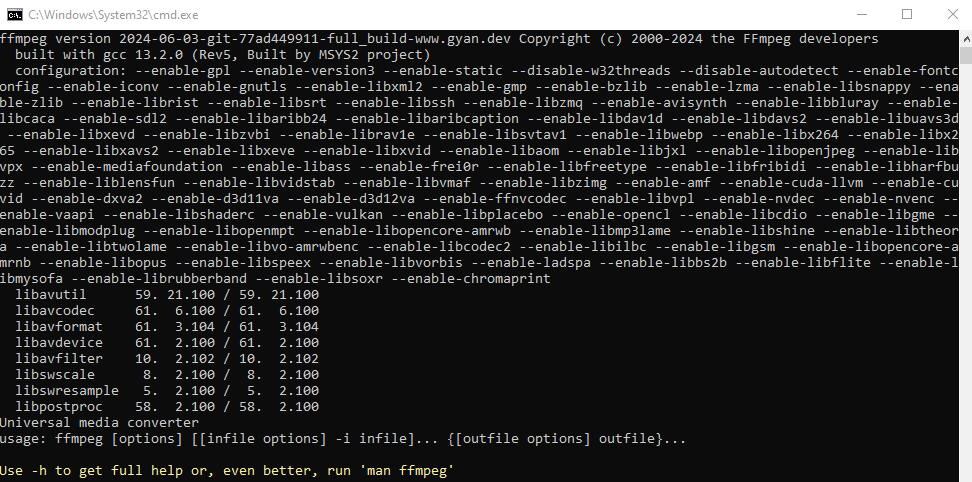
\includegraphics[width=0.85\linewidth]{img/ffmpeg.png}
    \caption{Comprobación de la instalación de \textit{Ffmpeg}}
    \label{fig:enter-label}
\end{figure}

\subsection{Ejecutar aplicación en local}
\subsubsection{Ejecución de aplicación Angular}
La ejecución de la aplicación Angular se puede hacer de dos maneras.
\begin{enumerate}
    \item Mediante el Angular CLI (Command Line Interface).
    \item Arrancar manualmente mediante el fichero \textit{package.json} del proyecto.
\end{enumerate}

Para realizar la ejecución mediante el Angular CLI seguiremos los siguientes pasos:
\begin{enumerate}
    \item Abrir terminal de comandos (cmd).
    \item Movernos a la raíz del proyecto Angular.
    \item Ejecutar el comando \textit{ng serve -o}. Con este comando ejecutaremos la aplicación y se abrirá directamente en el navegador en el puerto \textit{localhost:4200}.
\end{enumerate}

\begin{figure}[H]
    \centering
    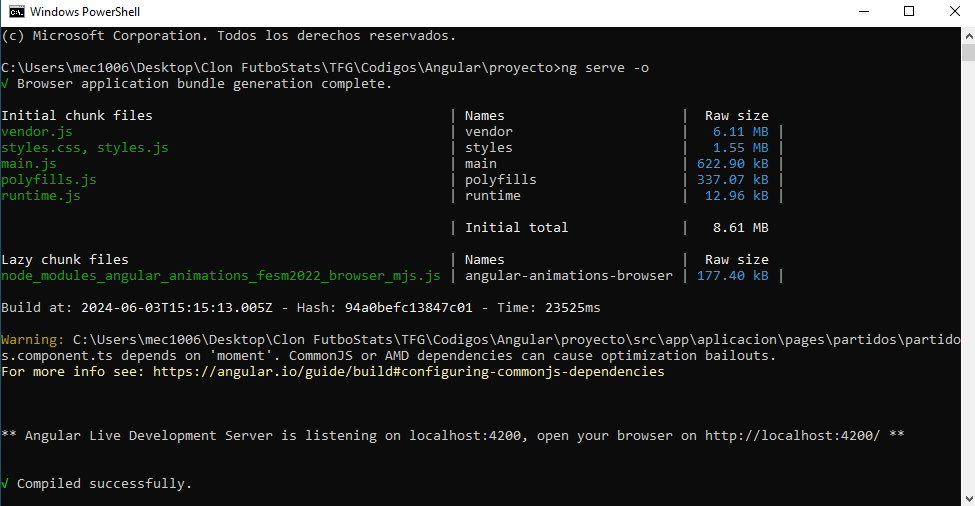
\includegraphics[width=0.85\linewidth]{img/ngserveCLI.png}
    \caption{Ejecución de la aplicación Angular mediante el comando \textit{ng serve -o} en el \textit{Angular CLI}.}
    \label{fig:enter-label}
\end{figure}

Para realizar la ejecución de la aplicación Angular desde Visual Studio Code seguiremos los siguientes pasos:
\begin{enumerate}
    \item Abrir el proyecto en Visual Studio Code.
    \item Abrir el fichero \textit{package.json}.
    \item Buscar la línea donde se encuentra el script \textit{ng serve -o}.
    \item Poner el cursor encima de \textit{start} y dar a \textit{Run Script}.
\end{enumerate}

\begin{figure}[H]
    \centering
    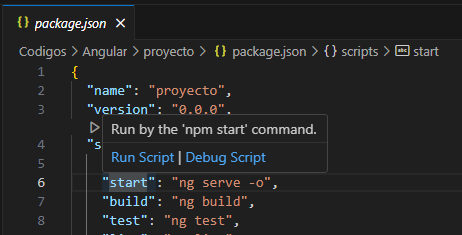
\includegraphics[width=0.85\linewidth]{img/ngserveVSC.png}
    \caption{Ejecución de la aplicación Angular desde Visual Studio Code.}
    \label{fig:enter-label}
\end{figure}

\subsubsection{Ejecución de aplicación Flask}
Para ejecutar la aplicación Flask usaremos el entorno virtual creado anteriormente. Para ello seguiremos los siguientes pasos:
\begin{enumerate}
    \item Abrir terminal.
    \item Movernos a la carpeta donde se encuentra el entorno virtual.
    \item Activar el entorno virtual en \textit{Flask/Scripts/activate}.
    \item Una vez activado el entorno virtual, nos movemos a la carpeta que contiene el fichero \textit{run.py} en \textit{Flask/run.py}.
    \item Ejecutamos la aplicación utilizando el comando \textit{python run.py}.
    \item La aplicación quedará disponible en \textit{http://127.0.0.1:5000}.
\end{enumerate}

\begin{figure}[H]
    \centering
    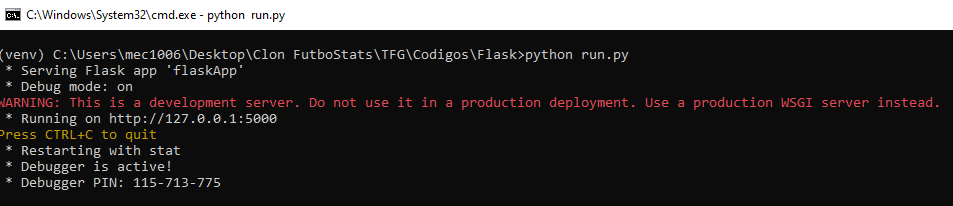
\includegraphics[width=0.9\linewidth]{img/ejecucionFlask.png}
    \caption{Ejecución de la aplicación Flask utilizando \textit{python run.py}}
    \label{fig:enter-label}
\end{figure}

\section{Pruebas del sistema}

Se han realizado pruebas de validación, pruebas de seguridad y pruebas de sistema para comprobar el correcto funcionamiento de la aplicación.

\subsection{Pruebas de validación}
Se han realizado validaciones de los formularios de consulta de datos de la siguiente manera:
\begin{itemize}
    \item Verificar que los formularios permiten seleccionar ligas, años, fechas, nombre del equipo y el resultado obtenido es correcto.
    \item Asegurar que los formularios manejan entradas incorrectas (se muestran mensajes de error en el caso de que no se introduzcan correctamente los parámetros de búsqueda).
    \item Validar que la información mostrada después de enviar el formulario es correcta y coincide con los datos esperados.
\end{itemize}

Se han realizado comprobaciones en la funcionalidad de subida y procesado de vídeos:
\begin{itemize}
    \item Probar funcionalidad de carga de vídeos mediante el explorador de archivos.
    \item Validar que los vídeos subidos son procesador correctamente y que se devuelve el vídeo procesado por ImageAI.
    \item Verificar que se manejen adecuadamente errores en la carga de archivos (formatos no soportados, archivos demasiado grandes).
\end{itemize}

Se han realizado pruebas respecto a las generación de gráficos y estadísticas:
\begin{itemize}
    \item Validar la correcta generación y visualización de gráficos generados en Python (mapas de calor, mapas de pases, mapas de posiciones, etc).
    \item Verificar que los modelos de goles esperados y puntos esperados generan resultados aproximados y coherentes con los datos proporcionados.
    \item Verificar que los gráficos se actualizan correctamente al cambiar el jugador seleccionado.
\end{itemize}

\subsection{Pruebas de seguridad}
Se han llevado acabo pruebas de autenticación, manejo de datos sensibles (claves API), autorización de API.

\begin{itemize}
    \item Verificar que el sistema requiere autenticación para acceder a las funcionalidades restringidas.
    \item Asegurar que los usuarios solo pueden acceder a los datos y funcionalidades para los que tienen permiso.
    \item Asegurar que datos como las claves API están protegidas y no se exponen al usuario.
    \item Verificar que las API utilizadas están correctamente autenticadas y autorizadas.
\end{itemize}

\subsection{Otras pruebas de sistema realizadas}
\begin{itemize}
    \item Medir el tiempo de respuesta para la consulta de datos y el envío de gráficos al \textit{front-end}.
    \item Probar la aplicación en diferentes navegadores (Chrome, Firefox, Edge, Safari) y dispositivos (escritorio, portátil, móvil) para comprobar su compatibilidad.
    \item Asegurar que la interfaz de usuario se muestra y funciona correctamente en todos los entornos probados.
    \item Evaluar la facilidad de uso de la interfaz de usuario, asegurándose de que los usuarios pueden navegar y realizar consultas de datos sin problemas.
    \item Asegurar que los diferentes componentes del sistema (\textit{front-end} en Angular, \textit{back-end} en Flask, procesamiento de vídeos con ImageAI, generación de gráficos con Python) se integran y funcionan correctamente juntos.
    \item Probar el flujo completo desde la entrada de datos en el formulario hasta la visualización de resultados y gráficos.
\end{itemize}

Estas pruebas ayudan a garantizar que la aplicación web sea robusta, segura y ofrezca una experiencia de usuario fluida y confiable.